\documentclass[../skript.tex]{subfiles}
\begin{document}

\begin{definition}[Minimal-/Maximalwinkelbedingung]\label{def:c2e5s3}
	Sei $\{\mathcal{T}_h\}_{h>0}$ eine Familie von regulären Triangulierungen (in 2D). $\{\mathcal{T}\}_h$ erfüllt die Minimal- (bzw. Maximal-) winkelbedingung, falls alle Winkel aller Triangulierungen von unten (bzw. von oben) durch eine konstante $\omega_{min}>0$ (bzw. $\omega_{max}>0$) beschränkt sind. 
\end{definition}
\begin{remark}\label{rem:c2e5s4}
	Eine Minimalwinkelbedingung impliziert auch eine Maximalwinkelbedingung.
\end{remark}

\begin{corollary}\label{cor:c2e5s5}
	Sei $\{\mathcal{T}_h\}_{h>0}$ eine Familie regulärer Triangulierungen, die der Maximalwinkelbedingung genüge, mit $\omega_{max}<\pi$. Dann gilt für jedes $h$ und jedes $v\in H^2(\Omega)$ die Beziehung
	\begin{IEEEeqnarray}{rcl}
		\|v-I_hv\|_{H^1(\Omega)} &\leq& \omega_{max} c(\omega_{max})\left( \sum_{T\in\mathcal{T}_h} h_T^2\|D^2v\|^2_{L^2(T)} \right)^{\frac{1}{2}} \\
		&\leq& c(\omega_{max}) h\|D^2v\|_{L^2(\Omega)}.
	\end{IEEEeqnarray}
\end{corollary}
\begin{remark}\label{rem:c2e5s6}
	Die Maximalwinkelbedingung in \cref{cor:c2e5s5} ist notwendig, siehe Übungsaufgabe 5.
\end{remark}
Zurück zum allgemeinen Fall $d\in\{1,2,3\},\,k\in\N$. Da die Abhängigkeit der Interpolationskonstanten von Formparametern der Elemente kompliziert ist, gehen wir zur Verallgemeinerung der Minimalwinkelbedingung über.
\begin{definition}\label{def:c2e5s7}
	Für jedes Element $T$ einer regulären Triangulierung $\mathcal{T}_h$ von $\Omega\subset\R^d$, definiere $\varrho>0$ als den Radius des größten in $T$ enthaltenen Balles. Dann charakterisiert der Quotient
	\[
		1 < \frac{h_T}{\varrho_T} < \infty
	\]
	die \emph{Degeneriertheit} des Elements $T$. \par
	Eine Familie $\{\mathcal{T}_h\}_{h>0}$ regulärer Triangulierungen heißt \emph{formregulär}, falls
	\[
		\sup_{h>0}\max_{T\in\mathcal{T}_h} \frac{h_T}{\varrho_T}\leq C,
	\]
	mit einer universellen Konstante $C>0$.
\end{definition}

\begin{figure}[ht]
	\centering
	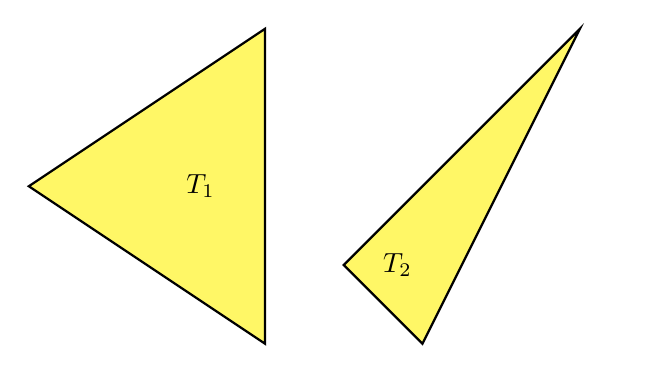
\begin{tikzpicture}
		\coordinate (A) at (0,0);
		\coordinate (B) at (3,2);
		\coordinate (C) at (3,-2);
		\coordinate (D) at (4,-1);
		\coordinate (E) at (5,-2);
		\coordinate (F) at (7,2);
		\draw[thick, fill=yellow!60] (A) -- (B) -- (C) -- (A) -- cycle;
		\draw[thick, fill=yellow!60] (D) -- (E) -- (F) -- (D) -- cycle;
		\node[text width=3cm] at (3.5,0) {$T_1$};
		\node[text width=3cm] at (6,-1) {$T_2$};
	\end{tikzpicture}
	\caption{Für $T_1$ ist der Quotient klein ( $|T|\equiv h_T^2$), für $T_2$ ist er hingegen groß ($|T| <<h_T^2$) }
\end{figure}
Das folgende Resultat ist eine direkte Konsequenz des Lemmas von \emph{Bramble und Hilbert}:\par
Sei $H^m(\Omega)$ ($m\in\N$) der Sobolevraum von $L^2$-Funktionen mit schwachen partiellen Ableitungen bis einschließlich Ordnung $m$ mit Norm
\[
	\|u\|_{H^m(\Omega)} \coloneqq \sqrt{\sum_{k=0}^m\|D^k u\|^2_{L^2(\Omega)}}.
\]
\begin{theorem}\label{thm:c2e5s8}
	Seo $\mathcal{T}_h$ eine reguläre Triangulierung von $\Omega$ und $k\in\N$. Dann gilt für alle $T\in\mathcal{T}_h$ und $v\in H^{k+1}(T)$, dass
	\[
		\|D^m(v-I_hv)\|_{L^2(T)} \leq C_{int}\left(\frac{h_T}{\varrho_T}\right)^k h_T^{k+1}\|D^k+1 v\|_{L^2}
	\]
	für alle $0\leq m\leq k+1$, wobei $C_{int}$ eine generische Konstante ist, die nur von $k,m$ und $\Omega$(?) abhängt, wobei
	\begin{IEEEeqnarray*}{rcl}
		I_h^k:H^2(\Omega)&\to& P^{k,0}(\mathcal{T}_h);\\
		I_h^kv\left( \sum_{h}(\mathcal{T}_h) \right) &=& v\left( \sum_h(\mathcal{T}_h) \right).
	\end{IEEEeqnarray*}
	Ferner gilt
	\begin{IEEEeqnarray*}{rcl}
		\|D^m(v-I_h^k v)\|_{L^2(\Omega)} &\leq& c_{int}\left(\max_{T\in\mathcal{T}_h}\frac{h_T}{\varrho_T} \right)^k\left( \sum_{T\in\mathcal{T}_h} h^{2(k+1-m)}\|D^{k+1}v\|_{L^2(T)}^2\right)^{\frac{1}{2}}\\
		&\leq& c_int\left( \max_{T\in\mathcal{T}_h}\frac{h_T}{\varrho_T} \right)^k h^{k+1-m} \|D^{k+1} v\|_{L^2(\Omega)} 
	\end{IEEEeqnarray*}
\end{theorem}
\begin{proof}
	Siehe \cite{Braess}.
\end{proof}

\section{Regularität schwacher Lösungen}\label{sec:c2e6}
Annahme für diesen Abschnitt: $\Gamma_D = \partial\Omega$, also $\Gamma_N = \emptyset$.
\begin{theorem}\label{thm:c2e6s1}
	Sei $\Omega$ konvex. Falls $u\in H^1_0(\Omega)$ mit $\Delta u\in L^2(\Omega)$, dann ist $u\in H^2(\Omega)$ und 
	\[
		\|D^2u\|_{L^2(\Omega)} \leq \|\Delta u\|_{L^2(\Omega)}.
	\]
\end{theorem}
\begin{proof}
	Siehe \cite{Grisvard}.
\end{proof}
\begin{theorem}\label{thm:c2e6s2}
	Sei $\Omega$ ein beschränktes Lipschitz-Gebiet mit glattem Rand ($\partial\Omega$ ist $ C^1$-Mannigfaltigkeit). Dann gibt es eine Konstante $C(\Omega)$, so dass für alle $u\in H^1_0(\Omega)$ mit $\Delta u\in L^2(\Omega)$, $u\in H^2(\Omega)$ und 
	\[
		\|D^2u\|_{L^2(\Omega)}\leq C(\Omega)\|\Delta u\|_{L^2(\Omega)}
	\]
	gilt.
\end{theorem}
\begin{theorem}\label{thm:c2e6s3}
	Sei $\Omega$ konvex und seien die hinreichenden Bedingungen für die Wohlgestelltheit von \cref{prb:c2e4s1} erfüllt (\cref{sec:c2e1}, \cref{thm:c2e2s7}). Außerdem sei $DA\in L^\infty(\Omega,\R^{d\times d\times d})$ und $f\in L^2(\Omega)$. Dann ist die eindeutige Lösung $u\in H^1_0(\Omega)$ von \cref{prb:c2e4s1} in $H^2(\Omega)$ und
	\[
		\|D^2u\|_{L^2(\Omega)} \leq C(\lambda,b,c,DA,\Omega)\|f\|_{L^2(\Omega)},
	\]
	wobei 
	\[
		C(\lambda,b,c,DA,\Omega) =  \lambda^{-2}(1-sqrt{2}\max\{\|b\|_{L^\infty}+\|DA\|_{L^\infty},\|c\|_{L^\infty}\})\left(1+\frac{(\meas{\Omega})^2}{\pi^2}\right)
	\]
\end{theorem}
\begin{proof}
	Folgt aus \cref{thm:c2e6s1}, \cref{thm:c2e2s7} und der Produktregel.
\end{proof}
\end{document}